\documentclass[tikz,convert=false,12pt]{standalone}
\renewcommand*\familydefault{\sfdefault} 
\renewcommand\familydefault{\sfdefault} 
\usepackage[T1]{fontenc}
\begin{document}
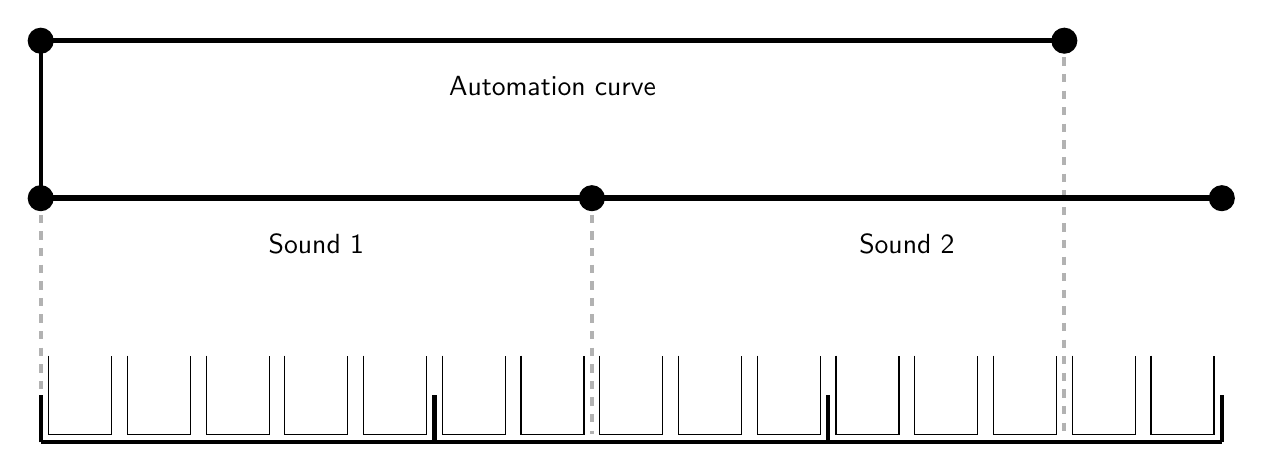
\begin{tikzpicture}
  \tikzstyle{event}=[circle,thick,fill=black];
  
    
  \draw [dashed, line width = 1.5, opacity=0.3] (0, 9) -- (0, 6) ;
  \draw [dashed, line width = 1.5, opacity=0.3] (7, 9) -- (7, 6) ;
  \draw [dashed, line width = 1.5, opacity=0.3] (13, 11) -- (13, 6) ;
  \draw [line width = 1.5, opacity=1] (0, 11) -- (0, 9) ;
    
  \coordinate (astart) at (0, 11);
  \coordinate (aend) at (13, 11);
  \draw [line width=2] (astart) -- (aend) node[midway,below,yshift=-3mm] {Automation curve};
  \node[event] at (astart) {};
  \node[event] at (aend) {};
  
  \coordinate (cstart) at (0, 9);
  \coordinate (cmid) at (7, 9);  
  \coordinate (cend) at (15, 9);    
  \draw [line width=2] (cstart) -- (cmid) node[midway,below,yshift=-3mm] {Sound 1};
  \draw [line width=2] (cmid) -- (cend) node[midway,below,yshift=-3mm] {Sound 2};
  \node[event] at (cstart) {};
  \node[event] at (cmid) {};
  \node[event] at (cend) {};
  
  
  % samples
  \foreach \x in {0,...,14}
    \draw [](0.1+\x, 7cm) -- (0.1+\x,6cm) -- (0.9+\x, 6cm) -- (0.9+\x,7cm);
  
  
  % ticks
  \foreach \x in {0,5,...,15}
    \draw [line width=1.5](\x, 5.9cm) -- (\x, 6.5cm) node[] {};
  \draw [line width=1.5](0, 5.9cm) -- (15, 5.9cm);
  
\end{tikzpicture}
\end{document}